% --------------------------------------------------------------

\documentclass[spanish, letterpaper,12]{article}

\usepackage[activeacute]{babel}
\usepackage[utf8x]{inputenc}
\usepackage[T1]{fontenc}
\spanishdecimal{.}

\usepackage{amsmath,amsthm,amssymb}
\usepackage[margin=1in]{geometry} 
\usepackage{graphicx}
\usepackage{hyperref}
\usepackage[numbers]{natbib}
\usepackage{enumitem} % para reducir el espacio [noitemsep,nolistsep]
\usepackage{verbatim}

\usepackage{mathtools}
\usepackage{booktabs} % para las tablas \toprule \bo

\DeclareGraphicsExtensions{.pdf,.png,.jpg}
\graphicspath{{./fig/}}


\usepackage{fancyhdr}
\renewcommand{\headrulewidth}{0pt}
\fancyhead[C]{
\includegraphics[width=3cm]{upa.jpg}}
\fancyhead[R]{}


\newcommand{\N}{\mathbb{N}}
\newcommand{\Z}{\mathbb{Z}}
 
\newenvironment{theorem}[2][Teorema]{\begin{trivlist}
\item[\hskip \labelsep {\bfseries #1}\hskip \labelsep {\bfseries #2.}]}{\end{trivlist}}
\newenvironment{lemma}[2][Lemma]{\begin{trivlist}
\item[\hskip \labelsep {\bfseries #1}\hskip \labelsep {\bfseries #2.}]}{\end{trivlist}}
\newenvironment{exercise}[2][Ejercicio]{\begin{trivlist}
\item[\hskip \labelsep {\bfseries #1}\hskip \labelsep {\bfseries #2.}]}{\end{trivlist}}
\newenvironment{problem}[2][Problema]{\begin{trivlist}
\item[\hskip \labelsep {\bfseries #1}\hskip \labelsep {\bfseries #2.}]}{\end{trivlist}}
\newenvironment{question}[2][Pregunta]{\begin{trivlist}
\item[\hskip \labelsep {\bfseries #1}\hskip \labelsep {\bfseries #2.}]}{\end{trivlist}}
\newenvironment{corollary}[2][Corollary]{\begin{trivlist}
\item[\hskip \labelsep {\bfseries #1}\hskip \labelsep {\bfseries #2.}]}{\end{trivlist}}



\begin{document}
 
% --------------------------------------------------------------
%                         Start here
% --------------------------------------------------------------
\title{Serie de Ejercicios}
\author{Profesor: Dr. Isaías Moreno Cruz\\
  Ingeniería en Energía Fototérmica (2023)\\
Universidad Politécnica de Aguascalientes (UPA)}
\date{18 de septiembre de 2023}

\maketitle

\begin{itemize}[leftmargin=*, noitemsep]
\item \textbf{Fecha de encargo:} lunes 18 de septiembre
\item \textbf{Fecha de entrega:} lunnes 25 de septiembre
\end{itemize}
% You can use theorem, exercise, problem, or question here.
% --------------------------------------------------------------
\thispagestyle{fancy}
\begin{problem}{1}
  Calcule la diferencia entre tiempo estándar y tiempo solar, en minutos, para la Ciudad de Obregón los días:
  \begin{itemize}[noitemsep]
    \item 21 de diciembre
    \item 21 de septiembre
    \item 21 de junio
  \end{itemize}

  Comente sus resultados.
\end{problem}

\begin{problem}{2}
  Calcule la posición solar, ángulos cenital $\theta_z$ y acimutal $\gamma_s$, así como el vector solar $\hat s$ para Temixco, Morelos. El día 25 de junio  a las 11:30 (tiempo solar).

\begin{figure}[ht]
  \centering
  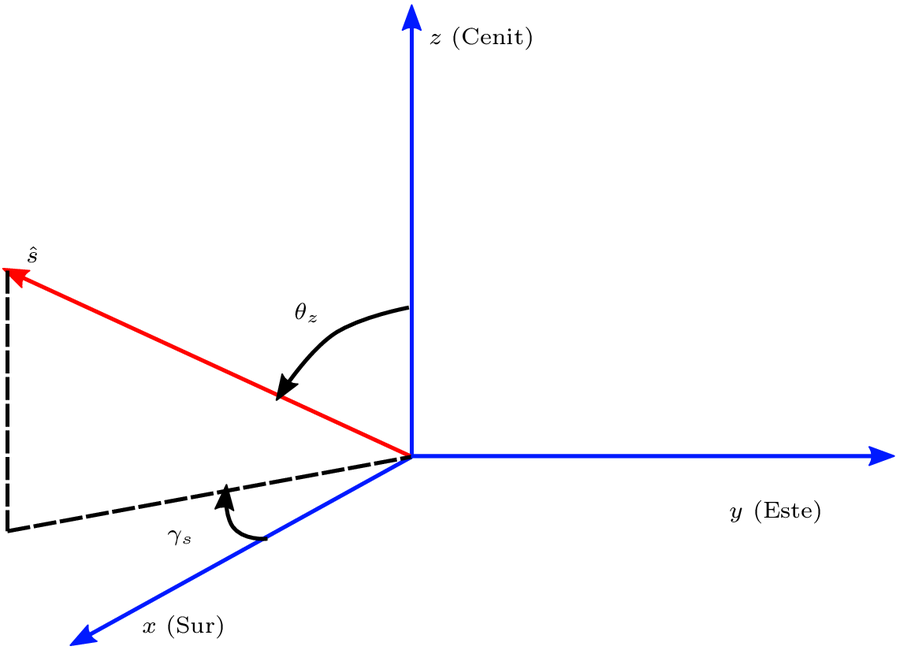
\includegraphics[width=0.35\textwidth]{vectorSolar}
  \caption{\label{fig:vectorSolar} Sistema de referencia de la posición solar.}
\end{figure}

\end{problem}

\begin{problem}{3}
A partir de la Ec.~\ref{eq:cos_theta} obtenga la ecuación para deducir la duración del día ($\omega_a$). Calcule cual es la duración del día el solsticio de invierno, verano y el equinoccio en las latitudes de 0, 15 y 30$^{\circ}$. ¿Donde se tiene el día más largo y por qué?

  \begin{equation}
    \label{eq:cos_theta}
    \cos(\theta_z) = \cos(\phi) \cos(\delta) \cos(\omega) +
    \sin(\phi) \sin(\delta)
  \end{equation}
\end{problem}

\begin{problem}{4}
  Para la barra mostrada en la Fig.~\ref{fig:barra} y la posición del vector solar dada por los ángulos $\theta_{z} = 5^{\circ}$ y $\gamma_{s} = - 15^{\circ}$, calcule:
  \begin{enumerate}[label=(\alph*)]
   \item El vector solar $\hat s$
   \item El ángulo $\xi$ que forma la sombra de una barra, orientada hacia el sur, con respecto a la horizontal.
    \end{enumerate}
  %% Para el 8 de dic a las 13hrs
  \begin{figure}[ht]
    \centering
    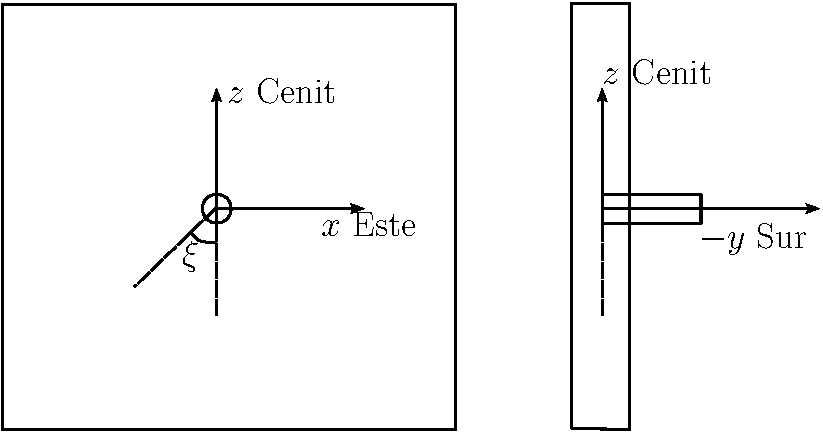
\includegraphics[width=0.4\textwidth]{barra}
    \caption{\label{fig:barra} Barra orientada hacia el sur.}
  \end{figure}
\end{problem}

\begin{problem}{5}
Para un colecto plano de 1.7 $m^2$ ubicado en Temixco calcula la potencia en que incide en el solsticio de verano al mediodía solar si la irradiancia es del 850 W/m$^{2}$:

\begin{itemize}
\item El colector horizontal que está orientado hacia el sur.
\item El colector esta inclinado la latitud del lugar, respecto a la horizontal y orientado hacia el sur.
\item El colector está inclinado 10 grados respecto a la horizontal y rotado 15 grados respecto al sur hacia el oeste.
\end{itemize}

\end{problem}


% \section*{Formulario}
% \label{sec:Formulario}
% % ----------------------------------------------------------------------

% \scriptsize

% \begin{align}
%   \label{eq:all}
%   &B[\text{grad}] = (n-1) \dfrac{360}{365} \\
%   &\begin{multlined}[b][.50\textwidth]
%       \label{eq:E}
%       E[\text{min}] = 229.2[0.000075 + 0.001868 \cos(B) -\\ 0.032077 \sin(B) - 0.014615 \cos(2B) - 0.04089 \sin(2B)]
%     \end{multlined}\\
%   &(\text{solar time} - \text{standard time}) [\text{min}] = 4(L_{st} - L_{loc}) + E, \quad \quad (0^\circ < L < 360^\circ)\\
%   &\delta[\text{grad}] = 23.45 \sin \left(360\dfrac{284+n}{365}\right)\\
%   &\cos(\theta_z) = \cos(\phi) \cos(\delta) \cos(\omega) + \sin(\phi) \sin(\delta)\\
%   & \tan \gamma_s = \dfrac{ \cos \delta \sin \omega }{\sin \phi \cos \delta \cos \omega - \cos \phi \sin \delta}\\
%   & \dot Q = G_b A \cos \theta\\
%   & \cos \theta = \cos \theta_z \cos \beta + \sin \theta_z \sin \beta \cos (\gamma_s - \gamma)
% \end{align}

% \begin{table}[h]
%   \centering
%   \scriptsize
%   \begin{tabular}[h]{lcc}
%     \toprule
%     & Temixco & Obregón\\
%     \midrule
%     latitud [grad], +Norte & 18.854 & 27.486\\
%     longitud [grad], +Oeste & 99.227 & 109.940\\
%     huso horario [hrs], +Oeste  & 6 & 7\\
%     \bottomrule
%   \end{tabular}
%   \caption{\label{tab:1} Latitud y longitud.}
% \end{table}

% % This LaTeX table template is generated by emacs 24.5.1
% \begin{table}[h]
%   \centering
%   \scriptsize
%   \begin{tabular}{lclc}
%         \toprule
%     Mes &  Día del año $n$  & Mes &  Día del año $n$  \\
%         & del $i$-ésimo día del mes &  & del $i$-ésimo día del mes \\
%         \midrule
%     Enero & $i$ & Julio & 181 + $i$ \\
%     Febrero & 31 + $i$ & Agosto & 212 + $i$ \\
%     Marzo & 59 + $i$ & Septiembre & 243 + $i$ \\
%     Abril & 90 + $i$ & Octubre & 273 + $i$ \\
%     Mayo & 120 + $i$ & Noviembre & 304 + $i$ \\
%     Junio & 151 + $i$ & Diciembre & 334 + $i$ \\
%     \bottomrule
%   \end{tabular}
%     \caption{\label{tab:2} Días promedio recomendados para calcular el día del año $n$.}
% \end{table}

\end{document}





